\documentclass[pra,12pt]{revtex4}
\usepackage{amsmath}
\usepackage{amssymb}
\usepackage{graphicx}
\usepackage{color}
\usepackage[pdfborder={0 0 0},colorlinks=true,linkcolor=blue,urlcolor=blue]{hyperref}

\def\ket#1{\left|#1\right\rangle}
\def\bra#1{\left\langle#1\right|}
\def\braket#1{\left\langle#1\right\rangle}

\usepackage{fancyhdr}
\fancyhf{}
\lhead{\tiny Y.~D.~Chong}
\rhead{\scriptsize PH4401: Quantum Mechanics III}
\lfoot{}
\rfoot{\thepage}
\pagestyle{fancy}

\setlength{\parindent}{14pt}
\renewcommand{\theequation}{A.\arabic{equation}}
\renewcommand{\thesection}{A\arabic{section}}

\renewcommand{\baselinestretch}{1.0}
\setlength{\parskip}{0.07in}

\begin{document}

\begin{center}
{\large \textbf{Appendix A: Circular and Spherical Waves}}
\end{center}

This Appendix describes the mathematics of circular waves and
spherical waves, and their use in 2D and 3D scattering problems.

\section{The Helmholtz equation}

Consider a non-relativistic particle moving in $d$-dimensional space
in the absence of a potential ($V = 0$), a scenario applicable to the
``exterior region'' of a scattering problem (Chapter 1).  The
time-independent Schr\"odinger equation is
\begin{equation}
  -\frac{\hbar^2}{2m}\nabla^2 \psi(\mathbf{r}) = E \psi(\mathbf{r}),
  \label{tise}
\end{equation}
where $\nabla^2$ denotes the $d$-dimensional Laplacian.  We will focus
on the $d = 2$ and $d = 3$ cases.

It is convenient to rewrite Eq.~\eqref{tise} as
\begin{equation}
  \Big(\nabla^2 + k^2\Big) \psi(\mathbf{r}) = 0,
  \label{helmholtz}
\end{equation}
where
\begin{equation}
  k = \sqrt{\frac{2mE}{\hbar^2}}.
  \label{kparm}
\end{equation}
The partial differential equation \eqref{helmholtz} is called the
\textbf{Helmholtz equation}.  We are interested in its solutions for
2D and 3D, with different choices of boundary conditions.

One class of elementary solutions is, of course, the plane waves
\begin{equation}
  \psi(\mathbf{r}) = \psi_0 \, \exp\left(i\mathbf{k}\cdot\mathbf{r}\right),
  \label{planewaves}
\end{equation}
where $\psi_0 \in \mathbb{C}$ and $\mathbf{k}$ is a $d$-component
vector satisfying $|\mathbf{k}| = k$ (where $k$ is the scalar
parameter in the Helmholtz equation).  The direction of $\mathbf{k}$
specifies the propagation direction.

In scattering problems, it is useful to turn to a different class of
solutions describing waves propagating outward (or inward) from a
point, instead of having a fixed direction like a plane wave.  Such
solutions can be constructed by going to polar coordinates $(r, \phi)$
for 2D, and spherical coordinates $(r,\theta,\phi)$ for 3D.

\section{Circular Waves in 2D}

In 2D polar coordinates $(r, \phi)$, the wavefunction has the form
\begin{equation}
  \psi(\mathbf{r}) = \psi(r,\phi).
\end{equation}
Since $\phi$ is an angular variable---i.e., $\psi(r,\phi + 2\pi) =
\psi(r, \phi)$---we can simplify the $\phi$ dependence by focusing on
harmonic solutions
\begin{equation}
  \psi(r,\phi) = \Psi_m(r)\, e^{im\phi}, \;\;\;m \in\mathbb{Z}.
  \label{psi_circular}
\end{equation}
More general solutions can be constructed from these, using
superpositions of different $m$.

Using Eq.~\eqref{psi_circular}, along with the expression for the 2D
Laplacian in polar coordinates,
\begin{equation}
  \nabla^2 = \frac{\partial^2}{\partial r^2} + \frac{1}{r} \,
  \frac{\partial}{\partial r} +
  \frac{1}{r^2}\frac{\partial^2}{\partial\phi^2},
\end{equation}
we obtain the following ordinary differential equation for $\Psi_m(r)$:
\begin{equation}
  r \frac{d}{dr}\!\left(r \frac{d\Psi_m}{dr} \right)
  + \Big(k^2 r^2 - m^2 \Big)\, \Psi_m(r) = 0.
  \label{besseleq}
\end{equation}
This is the Bessel equation, which supports the following solutions:
\begin{equation}
  \Psi_m(r) \propto \begin{cases}
    J_m(kr) &\text{(\href{https://docs.scipy.org/doc/scipy/reference/generated/scipy.special.jv.html}{Bessel function of the 1st kind})} \\
    Y_m(kr) &\text{(\href{https://docs.scipy.org/doc/scipy/reference/generated/scipy.special.yv.html}{Bessel function of the 2nd kind})} \\
    H_m^+(kr) \equiv J_m(kr) + i Y_m(kr) &\text{(\href{https://docs.scipy.org/doc/scipy/reference/generated/scipy.special.hankel1.html}{Hankel function of the 1st kind})} \\
    H_m^-(kr) \equiv J_m(kr) - i Y_m(kr) &\text{(\href{https://docs.scipy.org/doc/scipy/reference/generated/scipy.special.hankel2.html}{Hankel function of the 2nd kind})}.
  \end{cases}
\end{equation}
(Click on the links to refer to the implementations of these functions
in \href{https://scipy.org/}{Scientific Python}.)  The $J_m$ and $Y_m$
functions are real, while the $H_m^\pm$ functions are complex.
Notably, these four functions satisfy different boundary conditions in
the two limits $r\rightarrow 0$ and $r \rightarrow \infty$.

For $r \rightarrow 0$, $J_m$ is finite, while the others ($Y_m$ and
$H_m^\pm$) are divergent.

For $r \rightarrow \infty$, they have the following asymptotic forms:
\begin{align}
  \left.
  \begin{aligned}
    J_m(kr) &\rightarrow
    \sqrt{\frac{2}{\pi kr}} \cos\!\left(kr - \frac{m\pi}{2} - \frac{\pi}{4}\right) \\
    Y_m(kr) &\rightarrow
    \sqrt{\frac{2}{\pi kr}} \sin\!\left(kr - \frac{m\pi}{2} - \frac{\pi}{4}\right) \\
    H_m^+(kr) &\rightarrow
    \sqrt{\frac{2}{\pi kr}}
    \exp\left[i\left(kr - \frac{m\pi}{2} - \frac{\pi}{4}\right)\right] \\
    H_m^-(kr) &\rightarrow
    \sqrt{\frac{2}{\pi kr}}
    \exp\left[-i\left(kr - \frac{m\pi}{2} - \frac{\pi}{4}\right)\right]
  \end{aligned}\;\;
  \right\}
  \;\; \text{for}\;\, kr \rightarrow \infty,\;
  -\pi < \mathrm{arg}[kr] < \pi.
  \label{Jasymptote}
\end{align}
By analogy with Eq.~\eqref{planewaves}, we can interpret the Hankel
functions of the first kind as circular waves propagating
\textit{outward} from the origin, and the Hankel functions of the
second kind as circular waves propagating \textit{inward} to the
origin.  The Bessel functions are standing waves formed by a mix of
outgoing and incoming circular waves.

The prefactor of $1/\sqrt{r}$ in these aymptotic forms is consistent
with energy conservation.  In 2D, at radial distance $r$ the wave is
spread over a circumferential distance of $2\pi r$, so the combination
$|\Psi_m(r)|^2 \cdot 2\pi r$ is a constant.

We can convert between plane waves and circular waves with the help of
the identity
\begin{equation}
  e^{ikr\cos\phi} = \sum_{m=-\infty}^\infty i^m e^{im\phi} \, J_m(kr).
  \label{eikrcosphi}
\end{equation}

\section{Spherical Waves in 3D}
\label{sec:spherical}

Next, we consider solutions to the 3D Helmholtz equation expressed in
spherical coordinates $(r, \theta, \phi)$.  We can simplify the
dependence on the angular variables $\theta$ and $\phi$ by focusing on
wavefunctions of the form
\begin{equation}
  \psi(r,\theta,\phi) = \Psi_{\ell m}(r) \,Y_{\ell m}(\theta, \phi),
  \label{psi3d}
\end{equation}
where $Y_{\ell m}(\theta,\phi)$ denotes a
\href{https://docs.scipy.org/doc/scipy/reference/generated/scipy.special.sph_harm.html}{spherical
  harmonic} function.  In the context of quantum mechanics, such a
wavefunction has a definite angular momentum; $\ell$ and $m$ are the
quantum numbers for the total angular momentum and the $z$-component
of the angular momentum, respectively.  These are integers satisfying
\begin{equation}
  \ell \ge 0 \;\;\mathrm{and}\; -\ell\le m \le \ell,
\end{equation}
which ensures that $Y_{\ell m}(\theta,\phi)$ is both periodic in
$\phi$ and regular at the coordinate poles.

Upon plugging Eq.~\eqref{psi3d} into the Helmholtz equation, and
expressing the 3D Laplacian in spherical coordinates, we obtain the
following ordinary differential equation for $\Psi_{\ell m}(r)$:
\begin{equation}
  \frac{d}{dr}\left(r^2 \, \frac{d\Psi_{\ell m}}{dr}\right)
  + \Big[k^2r^2 - \ell(\ell+1)\Big] \Psi_{\ell m}(r) = 0.
  \label{sphbessel}
\end{equation}
Remarkably, the differential operator involves $\ell$ but \textit{not}
$m$.  Hence, the radial function depends only on $\ell$, and we will
henceforth write it as $\Psi_\ell(r)$ rather than $\Psi_{\ell m}(r)$.

Eq.~\eqref{sphbessel} has the following solutions:



two linearly independent real solutions,
$j_\ell(kr)$ and $y_\ell(kr)$, which are called \textbf{spherical
  Bessel functions}.  Most scientific computing packages provide
functions to calculate these; \href{https://scipy.org/}{Scientific
  Python}, for example, has
\href{https://docs.scipy.org/doc/scipy/reference/generated/scipy.special.spherical_jn.html}{\texttt{scipy.special.spherical\_jn}}
and
\href{https://docs.scipy.org/doc/scipy/reference/generated/scipy.special.spherical_yn.html}{\texttt{scipy.special.spherical\_yn}}.
Some spherical Bessel functions are plotted below:

\vskip 0.5cm
\begin{center}
  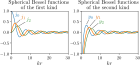
\includegraphics[width=0.67\textwidth]{spherical_bessel}
\end{center}

\noindent
Note that the $y_\ell$ functions diverge at $kr\rightarrow 0$.  This
does not bother us, for we are interested in solutions defined in the
exterior region, away from the coordinate origin.

For large values of the input, the spherical Bessel functions have the
limiting forms
\begin{align}
  \begin{aligned}j_\ell(kr)\; &\overset{kr\rightarrow\infty}{\longrightarrow} \; \frac{\sin(kr-\frac{\ell\pi}{2})}{kr} \\ y_\ell(kr)\; &\overset{kr\rightarrow\infty}{\longrightarrow} \; - \frac{\cos(kr-\frac{\ell\pi}{2})}{kr}.\end{aligned}
\end{align}
Since we are interested in incoming and outgoing spherical waves, it
is convenient to define
\begin{equation}
  h_\ell^\pm(kr) = j_\ell(kr) \pm i y_\ell(kr).
\end{equation}
This complex function is called a \textbf{spherical Hankel function}
of the first kind ($+$) or second kind ($-$).  It solves the same
differential equation, but has the limiting form
\begin{equation}
  h_\ell^\pm(kr)\; \overset{kr\rightarrow\infty}{\longrightarrow} \; \pm \frac{\exp\left[\pm i(kr-\frac{\ell\pi}{2})\right]}{ikr}.
\end{equation}
Using it, we can write down a solution to the Helmholtz equation, in
the form
\begin{equation}
  \Psi_{\ell m}^\pm(\mathbf{r}) = h_{\ell}^\pm(kr) \,Y_{\ell m}(\theta,\phi).
\end{equation}
This describes a spherical wave that is outgoing ($+$) or incoming
($-$), and that has a definite angular momentum described by the
quantum numbers $\ell$ and $m$.

Because the Helmholtz equation is linear, any linear combination of
spherical waves, with various values of $(\ell,m)$, is also a solution:
\begin{equation}
  \psi(\mathbf{r}) = \sum_\pm \sum_{\ell = 0}^\infty \sum_{m = - \ell}^\ell c_{\ell m}^\pm \Psi_{\ell m}^\pm(\mathbf{r}).
\end{equation}
It can be shown that the spherical waves form a complete solution
basis.  In other words, any solution to the 3D Helmholtz equation
within the exterior region can be written in the above form, for some
choice of complex coefficients $c_{\ell m}^\pm$.  (By the way, these
spherical waves are appropriately normalized so that the flux
associated with each term is directly proportional to $|c_{\ell
  m}^\pm|^2$.)

\section{The propagator}
\label{sec:propagator}

The propagator, introduced in Section 1.7, is the Green's function for
a free particle.  It is a solution to the partial differential
equation
\begin{equation}
  \Big(\nabla^2 + k^2\Big) \langle\mathbf{r} |\hat{G}_0 |\mathbf{r}'\rangle
  = \frac{2m}{\hbar^2} \; \delta^d(\mathbf{r}-\mathbf{r}').
\end{equation}
The left side of this equation is the same as the $d$-dimensional
Helmholtz equation \eqref{helmholtz}, with $\nabla^2$ acting on
$\mathbf{r}$ (not $\mathbf{r}'$), and $k$ given by Eq.~\eqref{kparm}.
On the right side, $\delta^d(\cdots)$ denotes a $d$-dimensional delta
function, and the prefactor of $2m/\hbar^2$ comes from how we defined
the Green's function by inverting the Hamiltonian (Section 1.6).

We can solve the differential equation with the help of the momentum
eigenbasis:
\begin{align}
  \langle\mathbf{r}|\hat{G}_0|\mathbf{r}'\rangle
  &= \langle\mathbf{r}|\hat{G}_0 \Big(\int d^dk' |\mathbf{k}'\rangle\langle\mathbf{k}'| \Big) |\mathbf{r}'\rangle \nonumber \\
  &= \int d^dk' \; \langle\mathbf{r}|\mathbf{k}'\rangle \;
  \frac{1}{E-\frac{\hbar^2|\mathbf{k}'|^2}{2m}} \;
  \langle\mathbf{k}'|\mathbf{r}'\rangle \nonumber \\
  &= \frac{2m}{\hbar^2} \frac{1}{(2\pi)^d} \int d^dk' \;
  \frac{\exp\left[i\mathbf{k}' \cdot
      (\mathbf{r}-\mathbf{r}')\right]}{k^2-|\mathbf{k}'|^2}.
  \label{rGr}
\end{align}
To calculate the $d$-dimensional integral, we must introduce an
explicit coordinate system.  In the following, we will show the
calculation for 3D.  The 2D case is left as an
\hyperref[ex:2dpropagator]{exercise}.

Take 3D spherical coordinates $(k',\theta,\phi)$, with the coordinate
axes aligned so that $\mathbf{r}-\mathbf{r}'$ points along the
$\theta=0$ direction.  We can now do the integral:
\begin{align}
  \langle\mathbf{r}|\hat{G}_0|\mathbf{r}'\rangle &= \frac{2m}{\hbar^2} \frac{1}{(2\pi)^3} \int d^3k' \; \frac{\exp\left[i\mathbf{k}'\cdot (\mathbf{r}-\mathbf{r}')\right]}{k^2-|\mathbf{k}'|^2} \nonumber \\
  &= \frac{2m}{\hbar^2} \frac{1}{(2\pi)^3} \int_0^\infty dk' \int_0^\pi d\theta \int_{0}^{2\pi} d\phi \;{k'}^{2}\sin\theta\; \frac{\displaystyle \exp\left(ik'|\mathbf{r}-\mathbf{r}'|\cos\theta\right)}{k^2-{k'}^2} \nonumber \\
  &= \frac{2m}{\hbar^2} \frac{1}{(2\pi)^2} \int_0^\infty dk' \int_{-1}^1 d\mu \;{k'}^2\; \frac{\displaystyle \exp\left(ik'|\mathbf{r}-\mathbf{r}'|\mu\right)}{k^2-{k'}^2} \qquad(\text{letting}\;\mu = \cos\theta) \nonumber \\
  &= \frac{2m}{\hbar^2} \frac{1}{(2\pi)^2} \int_0^\infty dk' \; \frac{ {k'}^2}{k^2-{k'}^2}\, \frac{\displaystyle \exp\left(ik'|\mathbf{r}-\mathbf{r}'|\right) - \exp\left(-ik'|\mathbf{r}-\mathbf{r}'|\right)}{ik'|\mathbf{r}-\mathbf{r}'|} \nonumber\\
  &= \frac{2m}{\hbar^2} \frac{1}{(2\pi)^2} \frac{i}{|\mathbf{r}-\mathbf{r}'|} \int_{-\infty}^\infty dk' \; \frac{\displaystyle k'\, \exp\left(ik'|\mathbf{r}-\mathbf{r}'|\right)}{(k' - k)(k'+k)}.
  \label{rGrintegrand}
\end{align}
This looks like something we can handle via contour integration.
However, there's a snag: the integration contour runs over the real
$k'$ line, but since $k \in \mathbb{R}^+$, the poles at $\pm k$ lie on
the contour.  The integral, as currently defined, is singular.

To make the integral non-singular, we must ``regularize'' it by
tweaking its definition.  One way is to displace the poles
infinitesimally in the complex $k'$ plane, shifting them off the
contour.  We have a choice of whether to move each pole
infinitesimally up or down.  It turns out that the appropriate choice
is to shift the pole at $-k$ down, and shift the pole at $+k$ up, as
illustrated by the red dots in the following figure:

\begin{figure}[h!]
  \centering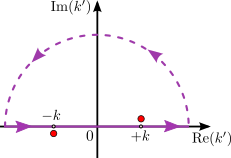
\includegraphics[width=0.37\textwidth]{greencontour}
\end{figure}

\noindent
This choice will yield a causal Green's function (Section 1.7).  It
alters the denominator in the integrand of Eq.~\eqref{rGrintegrand} as
follows:
\begin{equation}
  (k' - k)(k'+k) \;\rightarrow\; (k' - k - i\varepsilon)(k'+k+i\varepsilon) = {k'}^2 - (k+i\varepsilon)^2,
\end{equation}
where $\varepsilon$ is a positive infinitesimal.  This is equivalent
to replacing $E \rightarrow E + i\varepsilon$ in the definition of the
Green's function.  We can now do the integral:
\begin{align*}
  \begin{aligned}\int_{-\infty}^\infty dk' \; \frac{\displaystyle k' \exp\left(ik'|\mathbf{r}-\mathbf{r}'|\right)}{(k' - k)(k'+k)} &\rightarrow \lim_{\varepsilon \rightarrow 0^+} \int_{-\infty}^\infty dk' \; \frac{\displaystyle k' \exp\left(ik'|\mathbf{r}-\mathbf{r}'|\right)}{(k' - k - i\varepsilon)(k'+k+i\varepsilon)}\;\;\; (\text{regularize}) \\ &= \lim_{\varepsilon \rightarrow 0^+} \int_C dk' \; \frac{\displaystyle k' \exp\left(ik'|\mathbf{r}-\mathbf{r}'|\right)}{(k' - k - i\varepsilon)(k'+k+i\varepsilon)} \quad\;\;\; (\text{close contour above}) \\ &= 2\pi i \lim_{\varepsilon \rightarrow 0^+} \mathrm{Res}\left[\frac{\displaystyle k' \exp\left(ik'|\mathbf{r}-\mathbf{r}'|\right)}{(k' - k - i\varepsilon)(k'+k+i\varepsilon)}\right]_{k'=k+i\varepsilon^+} \\ &= \pi i \exp\left(ik|\mathbf{r}-\mathbf{r}'|\right).\end{aligned}
\end{align*}
Plugging this into Eq.~\eqref{rGrintegrand} yields
\begin{equation}
  \langle\mathbf{r}|\hat{G}_0|\mathbf{r}'\rangle = -\frac{2m}{\hbar^2}
  \cdot \frac{\exp\left(ik|\mathbf{r}-\mathbf{r}'|\right)}{4\pi|\mathbf{r}-\mathbf{r}'|},
\end{equation}
which describes a spherical wave propagating isotropically outward
from $\mathbf{r} = \mathbf{r}'$.  It is isotropic because the wave is
generated by a delta function, which has no preferred direction.  It
is outgoing due to our preceding choice of regularization.

The propagators for other spatial dimensions are given in Section 1.7.
The 1D and 2D derivations are very similar way to the above 3D
derivation.  The 2D case is left as an
\hyperref[ex:2dpropagator]{exercise}, with some hints provided.

\section{The scattering matrix}

For a given scattering problem, the exterior wavefunction is described
by the complex numbers $\{c_{\ell m}^+\}$ and $\{c_{\ell m}^-\}$.
These two sets of coefficients cannot, however, be independent of each
other.  For fixed $V(\mathbf{r})$ and $E$, suppose there is an
incoming spherical wave with definite angular momentum, say $c_{\ell
  m}^- = 1$ for some choice of $(\ell,m)$.  After striking the
scatterer, the quantum particle bounces back out to infinity, and the
outgoing wavefunction is some superposition of outgoing spherical
waves with a variety of angular momenta, described by certain
coefficients $\{c_{\ell' m'}^+\}$.

Thus, for each choice of incoming wave with definite angular momentum,
there is a corresponding set of outgoing-wave coefficients.  Since the
Schr\"odinger wave equation is linear, the principle of superposition
states that linear combinations of scattering solutions are also valid
solutions---i.e., solutions to the Schr\"odinger wave equation for the
same $V(\mathbf{r})$ and $E$.  So if we supply an \textit{arbitrary}
set of incoming coefficients $\{c_{\ell m}^-\}$, the outgoing
coefficients must be determined by a linear relation of the form
\begin{equation}
  c_{\ell m}^+ = \sum_{\ell'm'} S_{\ell m, \ell' m'} \;c_{\ell' m'}^-.
\end{equation}
To make the notation cleaner, we rewrite this as
\begin{equation}
  c_{\mu}^+ = \sum_{\nu} S_{\mu \nu} \, c_{\nu}^-,
\end{equation}
where each $\mu$ or $\nu$ denotes a pair of angular momentum quantum
numbers $(\ell,m)$, called a \textbf{scattering channel}.  The matrix
$S$ is called a \textbf{scattering matrix}.  Knowing $V(\mathbf{r})$
and $E$, we can calculate $S$, and knowing $S$ we can determine the
outgoing wavefunction produced by any set of incoming waves.

Thus far, we have not specified how the ``incoming'' and ``outgoing''
waves are related to the ``incident'' and ``scattered'' waves of a
scattering experiment.  We now consider an incident plane wave,
$\psi_i(\mathbf{r}) = \Psi_i \exp(i\mathbf{k}_i\cdot \mathbf{r})$,
where $|\mathbf{k}_i| = k$.  This introduces an important
complication: relative to the coordinate origin, a plane wave is
neither purely ``incoming'' nor ``outgoing''!  In fact, there is a
mathematical identity stating that
\begin{align}
  \begin{aligned}e^{i\mathbf{k}_i \cdot \mathbf{r}} &= \sum_{\ell=0}^\infty \sum_{m=-\ell}^\ell 4 \pi j_{\ell}(kr) e^{i\ell\pi/2} \, Y_{\ell m}^*(\hat{\mathbf{k}}_i) \, Y_{\ell m}(\hat{\mathbf{r}})\\ &= \sum_{\ell=0}^\infty \sum_{m=-\ell}^\ell 2 \pi \left[h_{\ell}^+(kr) + h_{\ell}^-(kr)\right] e^{i\ell\pi/2} \, Y_{\ell m}^*(\hat{\mathbf{k}}_i) \, Y_{\ell m}(\hat{\mathbf{r}}).\end{aligned}
  \label{plane_wave_decomp}
\end{align}
Here, $\hat{\mathbf{k}}_i$ denotes the angular components (in
spherical coordinates) of the incident wave-vector $\mathbf{k}_i$,
while $\hat{\mathbf{r}}$ likewise denotes the angular components of
the position vector $\mathbf{r}$.  Eq.~\eqref{plane_wave_decomp}
informs us that the incident plane wave can be decomposed into a
superposition of incoming and outgoing spherical waves, with the wave
coefficients
\begin{equation}
  c^{\pm}_{i, \ell m} = 2 \pi e^{i\ell\pi/2} \, Y_{\ell m}^*(\hat{\mathbf{k}}_i)\; \Psi_i.
\end{equation}
As described in Chapter 1, the total wavefunction in a scattering
problem is the sum of the incident wavefunction $\psi_i(\mathbf{r})$
and the scattered wavefunction $\psi_s(\mathbf{r})$.  The latter must
be a superposition of only outgoing spherical waves; let us denote the
coefficients by $c^+_{s,\ell m}$.  The scattering matrix relation can
then be re-written as
\begin{align}
  c^+_\mu &= c^+_{i,\mu} + c^+_{s,\mu} = \sum_{\mu\nu} S_{\mu\nu} c^-_{i,\nu} \\ \Rightarrow \;\;\; c^+_{s,\ell m} &= 2 \pi \sum_{\ell' m'} \Big(S_{\ell m, \ell' m'} - \delta_{\ell \ell'}\delta_{mm'}\Big) e^{i\ell'\pi/2} \, Y_{\ell' m'}^*(\hat{\mathbf{k}}_i)\; \Psi_i.
\end{align}
Using this, the scattered wavefunction can be written as
\begin{equation}
  \begin{aligned}\psi_s(\mathbf{r}) &= \sum_{\ell m} c^+_{s,\ell m} h_{\ell}^+(kr) \, Y_{\ell m}(\hat{\mathbf{r}}) \\ &= \Psi_i \sum_{\ell m} \sum_{\ell' m'} 2 \pi \Big(S_{\ell m, \ell' m'} - \delta_{\ell \ell'}\delta_{mm'}\Big) e^{i\ell'\pi/2} \, Y_{\ell' m'}^*(\hat{\mathbf{k}}_i)\; h_{\ell}^+(kr) \, Y_{\ell m}(\hat{\mathbf{r}}).\end{aligned}
\end{equation}
Taking the large-$r$ expansion of the spherical Hankel functions yields
\begin{equation}
  \psi_s(\mathbf{r}) \overset{r\rightarrow\infty}{\longrightarrow} \, \Psi_i \frac{e^{ikr}}{r} \; \left[ \frac{2 \pi}{ik}\, \sum_{\ell m} \sum_{\ell' m'} \Big(S_{\ell m, \ell' m'} - \delta_{\ell \ell'}\delta_{mm'}\Big) \, e^{-i(\ell-\ell')\pi/2} \, Y_{\ell' m'}^*(\hat{\mathbf{k}}_i)\; Y_{\ell m}(\hat{\mathbf{r}})\right].
\end{equation}
The quantity in square brackets is precisely what we call the
scattering amplitude:
\begin{equation}
  f(\mathbf{k}_i \rightarrow k\hat{\mathbf{r}}) =  \frac{2 \pi}{ik}\, \sum_{\ell m} \sum_{\ell' m'} \Big(S_{\ell m, \ell' m'} - \delta_{\ell \ell'}\delta_{mm'}\Big) \, e^{-i(\ell-\ell')\pi/2} \, Y_{\ell' m'}^*(\hat{\mathbf{k}}_i)\; Y_{\ell m}(\hat{\mathbf{r}}).
\end{equation}

\section{Spherically symmetric scattering potentials}

Generally, the scattering matrix needs to be calculated numerically.
The process is greatly simplified if the scattering potential is
spherically symmetric, i.e.~$V(\mathbf{r}) = V(r)$.  In that case,
angular momentum is conserved, so an incoming spherical wave with
angular momentum quantum numbers $(\ell,m)$ must scatter exclusively
into an outgoing spherical wave with the same $(\ell,m)$.  This means
that the scattering matrix components have the form
\begin{equation}
  S_{\ell m, \ell'm'} = s_{\ell m}\, \delta_{\ell\ell'}\, \delta_{mm'}.
\end{equation}
The scattering amplitude then simplifies to
\begin{equation}
  f(\mathbf{k}_i \rightarrow k\hat{\mathbf{r}}) =  \frac{2 \pi}{ik}\, \sum_{\ell m} \Big(s_{\ell m} - 1\Big) \, Y_{\ell m}^*(\hat{\mathbf{k}}_i)\; Y_{\ell m}(\hat{\mathbf{r}}).
\end{equation}

Our task is now to obtain the $s_{\ell m}$'s.  The procedure is very
similar to what we already went through in
\textcolor{red}{Section~\ref{sec:spherical}}.  The total wavefunction satisfies the
Schr\"odinger wave equation, which can be written in spherical
coordinates as
\begin{equation}
  \frac{1}{r^2}\frac{\partial}{\partial r}\left(r^2\frac{\partial \psi}{\partial r}\right) + \frac{1}{r^2\sin\theta}\frac{\partial}{\partial\theta}\left(\sin\theta\frac{\partial\psi}{\partial\theta}\right)+\frac{1}{r^2\sin^2\theta}\frac{\partial^2\psi}{\partial\phi^2} + K^2(r) \psi(r,\theta,\phi) = 0,
\end{equation}
where
\begin{equation}
  K^2(r) = \sqrt{\frac{2m\big[E-V(r)\big]}{\hbar^2}}.
\end{equation}
This is similar to the Helmholtz equation, but with the constant $k^2$
replaced by a function $K^2(r)$.  In scattering channel $(\ell,m)$,
the solution has the form
\begin{equation}
  \psi(r,\theta,\phi) = A(r) \, Y_{\ell m}(\theta, \phi).
\end{equation}
Upon substitution into the Schr\"odinger wave equation, we find that
$A(r)$ must satisfy
\begin{equation}
  \frac{d}{dr}\left(r^2\frac{dA}{dr}\right) + \Big[K^2(r)\, r^2 - \ell(\ell+1)\Big] A(r) = 0, \;\;\;\ell \in \mathbb{Z}_0^+.
\end{equation}
As before, the equation for $A(r)$ does not involve $m$; hence, the
scattering matrix components do not depend on $m$, and can be written
as simply
\begin{equation}
  s_{\ell m} \,=\, s_\ell.
\end{equation}
For any given $V(r)$, we can solve the second-order ordinary
differential equation numerically by supplying two boundary conditions
at $r=0$, integrating up to a large value of $r$, and matching to the
exterior solution
\begin{equation}
  A(r) \; \overset{r\rightarrow\infty}{\longrightarrow} \; c^-_\ell h^-_\ell(kr) + c^+_\ell h^+_\ell(kr) = c^-_\ell \Big(h^-_\ell(kr) + s_\ell h^+_\ell(kr)\Big).
\end{equation}
The value of $s_\ell$ can then be extracted.

To simplify the problem even further, let the scattering potential
take the form of a spherical potential well of radius $R$ and depth
$U$:
\begin{equation}
  V(r) = \begin{cases}-U &\mathrm{for}\;\; r < R, \\ \;\;\; 0 & \mathrm{otherwise}.\end{cases}
\end{equation}
We will take $U > 0$, so that the potential is attractive.  (The
interested reader can work through the repulsive case, $U < 0$.  The
process is almost the same as what is presented below, except that for
some values of $E$, the wave inside the scatterer becomes evanescent.)
Now, the Schr\"odinger wave equation in the interior region reduces to
the Helmholtz equation, but with $k$ replaced with
\begin{equation}
  q = \sqrt{2m(E+U)/\hbar^2}.
\end{equation}
Note that $q \in \mathbb{R}^+$ for $E > 0$, since we have assumed
that $U > 0$.  The elementary solutions for $A(r)$ in the interior
region are $j_\ell(qr)$ and $y_\ell(qr)$.  However, we must exclude
the latter, since they diverge at $r = 0$.  (When we got to a similar
point in Section~\ref{sec:spherical}, we did not exclude the spherical
Bessel functions of the second kind, because at the time we were
concerned with solutions in the exterior region.)  We thus arrive at a
solution of the form
\begin{equation}
  A(r) = \begin{cases} \alpha_\ell\, j_\ell(qr), & r \le R \\ c^-_\ell \Big(h^-_\ell(kr) + s_\ell h^+_\ell(kr)\Big) & r \ge R.\end{cases}
\end{equation}
So far, the values of $\alpha_\ell$, $c^-_\ell$, and $s_\ell$ remain
unknown.  To proceed, we match the wavefunction and its
derivative at the boundary $r = R$:
\begin{align}
  \begin{aligned} \alpha_\ell\, j_\ell(qR) &= c^-_\ell \Big(h^-_\ell(kR) + s_\ell h^+_\ell(kR)\Big) \\ \alpha_\ell\, q j_\ell'(qR) &= c^-_\ell k \Big({h^-_\ell}'(kR) + s_\ell {h^+_\ell}'(kR)\Big).\end{aligned}
\end{align}
Here, $j_\ell'$ denotes the derivative of the spherical Bessel
function, and likewise for ${h_\ell^\pm}'$.  Taking the ratio of these
two equations eliminates $\alpha_\ell$ and $c_\ell^-$:
\begin{equation}
  \frac{q j_\ell'(qR)}{j_\ell(qR)} = k \frac{{h^-_\ell}'(kR) + s_\ell {h^+_\ell}'(kR)}{h^-_\ell(kR) + s_\ell h^+_\ell(kR)}.
\end{equation}
With a bit of rearrangement, this becomes
\begin{equation}
  s_\ell = - \frac{k{h_\ell^-}'(kR) j_\ell(qR) - qh_\ell^-(kR)j_\ell'(qR)}{k{h_\ell^+}'(kR) j_\ell(qR) - qh_\ell^+(kR)j_\ell'(qR)}.
\end{equation}
The numerator and denominator are complex conjugates of one another,
since $j_\ell$ is real and $(h_\ell^+)^* = h_\ell^-$.  Hence,
\begin{equation}
  s_\ell = e^{2i\delta_\ell}, \;\;\;\mathrm{where}\;\; \delta_\ell = \frac{\pi}{2} - \mathrm{arg}\!\left[k{h_\ell^+}'(kR) j_\ell(qR) - qh_\ell^+(kR)j_\ell'(qR)\right].
\end{equation}
In other words, the scattering matrix component is a pure phase
factor.  This is actually a consequence of energy conservation.  Since
the scattering matrix does not couple different angular momentum
channels (due to the spherical symmetry), the incoming flux and
outgoing flux in each channel must be equal.  Hence, the only thing
the scattering potential can do is to shift the phase of the outgoing
spherical wave component in each channel.

Once we find $\delta_\ell$, we can compute the scattering amplitude
\begin{equation}
  f(\mathbf{k}_i\rightarrow k\hat{\mathbf{r}}) = \frac{2 \pi}{ik}\, \sum_{\ell =0}^\infty \big(e^{2i\delta_\ell} - 1\big) \, \sum_{m=-\ell}^\ell \,Y_{\ell m}^*(\hat{\mathbf{k}}_i)\; Y_{\ell m}(\hat{\mathbf{r}}).
\end{equation}
This can be simplified with the aid of the following addition theorem
for spherical harmonics:
\begin{equation}
  P_\ell(\hat{\mathbf{r}}_1\cdot\hat{\mathbf{r}}_2) = \frac{4\pi}{2\ell+1} \sum_{m=-\ell}^{\ell} Y_{\ell m}^*(\hat{\mathbf{r}}_1) Y_{\ell m}(\hat{\mathbf{r}}_2).
\end{equation}
where $P_\ell(\cdots)$ denotes a
\href{https://en.wikipedia.org/wiki/Legendre_polynomials}{Legendre
  polynomial}.  We finally obtain
\begin{equation}
  \boxed{\quad\begin{aligned}f(\mathbf{k}_i \rightarrow k\hat{\mathbf{r}}) &= \frac{1}{2ik}\, \sum_{\ell =0}^\infty \big(e^{2i\delta_\ell} - 1\big) \big(2\ell+1\big)\, P_{\ell}(\hat{\mathbf{k}}_i\cdot \hat{\mathbf{r}}) \\ \delta_\ell &= \frac{\pi}{2} - \mathrm{arg}\!\left[k{h_\ell^+}'(kR) \, j_\ell(qR) - qh_\ell^+(kR)\, j_\ell'(qR)\right] \\ k &= |\mathbf{k}_i| = \sqrt{2mE/\hbar^2}, \;\; q = \sqrt{2m(E+U)/\hbar^2}.\end{aligned}\quad}
\end{equation}
This result for the scattering amplitude depends upon two variables:
(i) $E$, the particle energy (which is conserved), and (ii) $\Delta
\theta = \cos^{-1}(\hat{\mathbf{k}}_i\cdot \hat{\mathbf{r}})$, the
\textbf{deflection angle} (i.e., the angle between the direction of
incidence and the direction into which the particle is scattered).

\section*{Exercises}

\begin{enumerate}
\item \label{ex:2dpropagator}
  In Section~\ref{sec:propagator}, we derived the 3D propagator.
  Using a similar procedure, prove that the 2D propagator is
  \begin{equation}
    \langle\mathbf{r}|\hat{G}_0|\mathbf{r}'\rangle = \frac{2m}{\hbar^2}\;
    \cdot\; \frac{1}{4i} H^+_0(k|\mathbf{r}-\mathbf{r'}|).
  \end{equation}
  In evaluating the polar integral, you may find it useful to invoke
  Eq.~\eqref{eikrcosphi}.  To solve the resulting contour integral,
  you may refer to the asymptotic forms of the Bessel and Hankel
  functions given in \eqref{Jasymptote}, and the identity
  \begin{equation}
    H_m^+(z) = - (-1)^m \, H_m^-(-z).
  \end{equation}

  

\end{enumerate}

\end{document}
